\chapter{Implementação}
A implementação do sistema segue todas as diretrizes de tecnologias e conceitos apresentados até este tópico. A descrição de como a implementação foi feita será dividida em duas partes principais: \textit{backend} e \textit{frontend}. Sendo a parte de \textit{backend} a implementação da infraestrutura e servidor da aplicação, e na parte do \textit{frontend} a implementação de interface com o usuário. No desenvolvimento elegemos um nome fictício para a aplicação, chamado Orb. Este nome será utilizado para remeter a aplicação em alguns textos, logos, implementações, entre outros.

O código-fonte da aplicação está hospedado no GitHub \cite{orb}, como \textit{software open-source}, liberado para utilização através da licença MIT \cite{mit}. A abordagem utilizada para a descrição da implementação feita fará referências pontuais a trechos do código-fonte que poderão ser consultados pelo leitor no repositório informado \cite{orb}, evitando-se assim a exposição de código neste formato de texto que não é favorável a análise deste tipo de conteúdo.

\section{Backend}
Primeiramente iremos descrever a criação do ambiente de desenvolvimento do projeto, onde inicialmente foi instalado o sistema operacional e todas as ferramentas que decidimos utilizar para a construção da aplicação, e posteriormente iniciamos o processo de codificação.

Iniciando-se pelo sistema operacional, foi criada uma partição separada no disco rígido, com volume de 60 GBs. O sistema operacinal escolhido para o ambiente de desenvolvimento foi de uma distribuição Linux chamada CentOS \cite{centos}, versão 7. A instalação do sistema operacional foi feita através de um \textit{pendrive} e foram seguidas todas as configurações padrões do \textit{wizard} de instalação do sistema.

Após a instalação do sistema operacional, foi feita a instalação de todas as ferramentas que foram escolhidas para o desenvolvimento da aplicação, como o NodeJS, MongoDB, Redis, editores de texto e navegadores. Todas estas ferramentas foram instaladas através do repositório de pacotes padrão do sistema CentOS 7, chamado YUM. Para algumas ferramentas foram necessário a atualização das fontes do repositório YUM e outras foram instaladas através de pacotes RPM (Red Hat Package Manager ou RPM Package Manager) disponibilizados no próprio site da ferramenta.

A implementação do \textit{backend} iniciou-se com a criação de um diretório chamado backend na pasta raiz do projeto, do qual a partir dele foram seguidas recomendações de boas práticas \cite{express-app-structure} para a organização da estrutura de diretórios em aplicações ExpressJS. A seguinte listagem identifica o nome destes diretórios e suas respectivas funcionalidades:

\begin{description}
	\item[controllers] Este diretório contém os arquivos de código relacionados as rotas e suas lógicas de implementação. Rotas são os \textit{endpoints} que podem ser acessados através de requisições HTTP enviadas por uma determinada URL que a identifica. Neste diretório contém os arquivos das rotas de cliente, usuário e \textit{token}.
	
	\item[domain] Este diretório contém os arquivos relacionados a lógica de negócio da aplicação. Os \textit{handlers} que tratam as requisições \textit{websocket} da aplicação estão implementados em arquivos contidos nesta pasta.
	
	\item[helpers] Este diretório contém arquivos que implementam funcionalidades que podem ser utilizadas em diversos pontos do sistema, este diretório funciona como um \textit{cross-cutting layer} da aplicação. Nesta pasta estão implementados alguns métodos que ajudam na geração de \textit{random strings} e retorno de \textit{datetime} em formato UTC (Coordinated Universal Time).
	
	\item[middlewares] Este diretório contém arquivos relacionados a \textit{middlewares} de tratamento de requisições que chegam ao servidor, como realização de autenticação e autorização de acesso as rotas da aplicação.
	
	\item[models] Este diretório contém arquivos relacionados aos objetos que podem ser persistidos na aplicação. Devido ao Javascript ser uma linguagem dinâmica, estes objetos não representam um contrato de como estes eles devem existir na aplicação, mas como eles devem ser persistidos no banco de dados, que no caso desta aplicação é o MongoDB. Neste diretório serão encontrados os arquivos de persistência dos \textit{tokens}, \textit{chat}, \textit{messages}, \textit{users}, entre outros.
\end{description}

Após a definição da estrutura de diretórios da aplicação, foi realizada a instalação e inicialização do NPM, responsável por gerenciar todos os pacotes que iremos utilizar no desenvolvimento da solução.

\subsection{Persistência}
A persistência dos dados foi feita em um banco de dados MongoDB, onde para sua utilização foi feito o \textit{download} doo pacote Mongoose pelo NPM. A conexão com o banco foi feita no arquivo de inicialização da aplicação, através do método connect do próprio Mongoose, passando-se como parâmetros uma \textit{connection string} com o endereço local do banco de dados. Por ser um ambiente de testes, não utilizamos autenticação com o banco de dados, mas caso fosse necessário, bastava-se apenas adicionar os dados de \textit{username:password} na própria \textit{connection string}.

No diretório \textit{models} foram criados arquivos para cada objeto que fosse ser persistido no banco. As implementações da persistência utilizaram o Mongoose como modelo, exportando de cada módulo o objeto \textit{schema} de cada persistência, podendo através deste realizar todas as operações de CRUD (Create, Read, Update, Delete).

A seguinte imagem ilustra a representação dos objetos persistidos no banco de dados:

\begin{figure}[!htb]
	\centering
	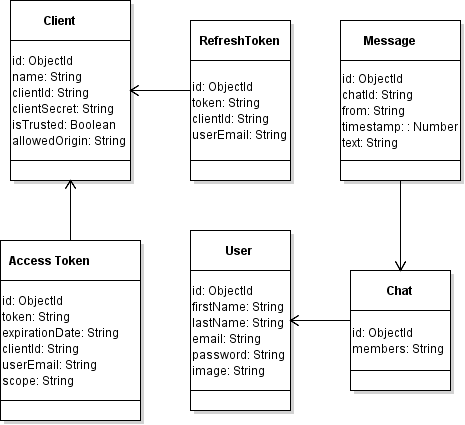
\includegraphics[scale=0.85]{imagens/models_uml.png}
	\caption{\small Representação UML (Unified Modeling Language) dos modelos persistidos no banco de dados.}
	\label{fig:modelsuml}
\end{figure}


\subsection{Autenticação e Autorização}
Para a implementação do sistema de autenticação, cujos códigos estão no diretório middlewares, utilizamos três pacotes NPM, que funcionam como \textit{middlewares} que extraem de um \textit{request} as informações de autenticação, e através de uma \textit{callback} é possível validar essas informações e sinalizar se as informações estão corretas para concretização da autenticação. Para o sistema de autorização, utilizamos o OAuth2 com algumas modificações em seu padrão para atender aplicações \textit{trusted}, como o nosso \textit{frontend app} desenvolvido em AngularJS, que é um tipo de aplicação que não necessita de autorização do usuário da conta para acessar suas informações confidenciais.

Como estamos utilizando um sistema de \textit{tokens}, para realizar acesso ao \textit{endpoint} token, o qual é utilizado no sistema de \textit{login} para se conseguir um Access Token e um Refresh Token através do fornecimento de \textit{e-mail} e senha, é realizada a autenticação pelos padrões Basic \cite{passport-basic} e Client \cite{passport-client}. Após esta autenticação, o usuário é encaminhado para um \textit{exchange} do OAuth2 que irá gerar, persistir e retornar um Access Token e um Refresh Token para o solicitante, que poderá usá-lo para acessar os demais \textit{endpoints} da aplicação.

Como já introduzido, o restante dos das rotas da aplicação são protegidos através do padrão de autenticação Bearer \cite{passport-bearer}, que procura em cada requisição feita um Access Token, que será verificado, e caso seja válido permitirá o acesso ao \textit{endpoint} solicitado. Em caso do Access Token não ser válido, o servidor irá emitir uma resposta de erro, HTTP 401, informando o problema ocorrido, e se o problema for a expiração do Access Token, ele poderá utilizar o Refresh Token para conseguir um novo Access Token válido por mais um determinado tempo, evitando de ter que realizar toda o processo de autenticação com \textit{e-mail} e senha novamente.

\begin{figure}[!htb]
	\centering
	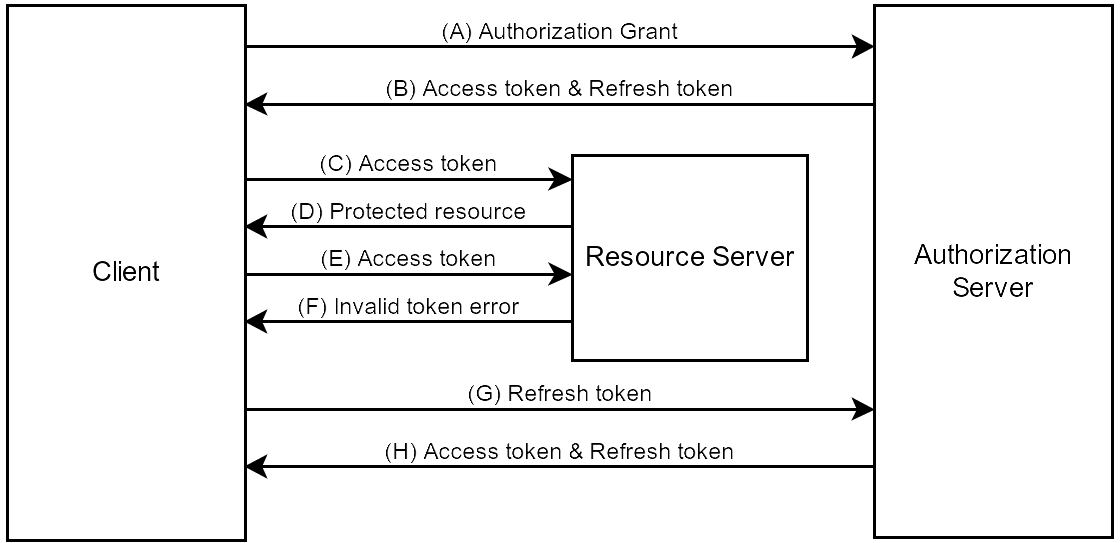
\includegraphics[scale=0.49]{imagens/oauth2.png}
	\caption{\small Fluxo de acesso aos recursos com OAuth2. Fonte: jlabusch \cite{img-jlabusch}}
	\label{fig:oauth2}
\end{figure}

Um detalhe importante que deve ser falado, é a utilização do método bcrypt \cite{bcrypt} para criptografia da senha dos usuários e a utilização do crypt \cite{crypt} para a criptografia do Access Token e Refresh Token. Como o bcrypt é um tipo de criptografia mais complexa, que leva em conta o custo de processamento, utilizamos-o em funcionalidades menos requisitadas, como o \textit{login}, e utilizamos o crypt (SHA256) para a criptografia dos \textit{tokens}, pois são requisitados na maioria das rotas do sistema, consequentemente necessitando-se fazer a verificação de chaves a todo momento, sendo assim, a utilização de um método menos custoso se faz benéfico.

\subsection{Rotas}
As rotas de aplicação estão organizadas no diretório controller da aplicação, tendo sido implementadas de acordo com o tipo de persistência que elas representam. A seguir, uma listagem organizada pelos \textit{endpoints} das rotas e uma descrição sobre sua funcionalidade:

\begin{description}
	\item[client] A rota client possui dois \textit{endpoints} que podem ser acessados através de chamadas pelo método HTTP GET e HTTP POST. O método GET retorna uma lista em formato JSON de todos os clients cadastrados no sistema. O método POST recebe um client em formato JSON e cadastra-o no banco.
	
	\item[token] A rota token possui apenas um \textit{endpoint} chamado revoke, o qual é responsável por remover do banco de dados o Access Token e Refresh Token relacionados a um determinado cliente. Este \textit{endpoint} é utilizado para realizar o \textit{signout} da aplicação.
	
	\item[user] A rota user possui quatro \textit{endpoints}, sendo o primeiro podendo ser chamado pelo método GET e retornando todos os usuários persistidos. O segundo pelo método GET, passando-se como parâmetro o id do usuário que se quer retornar. O terceiro pelo método POST, passando-se como parâmetro o usuário em formato JSON que se quer persistir. O quarto pelo \textit{endpoint} accesstoken e método GET, passando-se como parâmetro o Access Token do usuário que se quer retornar.
\end{description}

As rotas seguem o padrão de utilização dos métodos HTTP para realização do CRUD em APIs, sendo os \textit{endpoints} citados funcionalidades da aplicação, e são protegidos de acordo com as especificações faladas no tópico Autenticação e Autorização. Estes \textit{endpoints} são chamados pela aplicação \textit{frontend}, que passa em cada \textit{request} todas as informações de autenticação necessária, e trata os dados de sucesso ou erro que cada \textit{endpoint} retorna.

\subsection{Socket}
O desenvolvimento da comunicação em tempo real do \textit{chat} é a principal funcionalidade do \textit{backend} da aplicação. Os arquivos de implementação estão localizados no diretório domain, onde três arquivos implementam todas as funcionalidades relacionadas.

Inicialmente foi feito o \textit{download} pelo NPM das bibliotecas socket.io e redis. A inicialização do servidor de conexão do socket.io foi feita no arquivo de inicialização do servidor através da porta 1200. A conexão com o banco de dados Redis foi feita no arquivo que trava os eventos dos \textit{sockets}.

Com a biblioteca devidamente configurada, o servidor já está pronto para receber conexões \textit{socket}. No arquivo socketBootstrap.js criamos um sistema de inicialização que cria um \textit{namespace} de conexão chamado chat, e também realiza a autenticação dos usuários que tentam estabelecer uma conexão por \textit{socket} com o servidor. Para tratar a autenticação, utilizamos uma biblioteca \cite{socketio-auth} que oferece uma solução semelhante a explicada no tópico Autenticação e Autorização.

No arquivo chatSocketHandler.js implementamos todos os eventos de envio e recebimento de mensagens dos \textit{sockets}. Visando a utilização do protocolo PUB/SUB, abrimos três conexões/canais com o nosso servidor Redis, o primeiro para \textit{publish} de mensagens, o segundo para \textit{subcription} e o terceiro para \textit{storage} de informações dos usuários \textit{online}.

A seguir uma lista dos eventos emitidos e recebidos no \textit{namespace} chat e a descrição de seu funcionamento:

\begin{description}
	\item[disconnect] Este evento é emitido por um cliente que se desconectou do servidor. Neste evento tratamos de remover este usuário da lista de usuários \textit{online} do \textit{storage} e lançamos um evento chat:signout, comunicando a todos os usuários que aquele usuário se desconectou, logo devem o remove-lo de seu mapa.
	
	\item[chat:signout] Este evento é emitido para todos os usuários, informando-os o id de um usuário que acabou de se desconectar do servidor. Quando este evento é recebido pelo cliente, ele procura e remove este usuário do seu mapa.
	
	\item[chat:new] Este evento é emitido pelo cliente quando ele inicia um \textit{chat} com outro usuário. Este evento procura no banco de dados a existência de uma conversa entre os dois usuários, caso exista, esta conversa é lida com as últimas 15 mensagens registradas. Caso não exista, é criada uma nova conversa entre os usuários.
	
	\item[chat:online:list] Este evento é recebido pelo servidor e emitido por ele próprio com uma lista de informações de todos os usuários \textit{online}, inclusive suas respectivas localizações geográficas.
	
	\item[chat:message:send] Este evento é emitido pelo cliente quando ele clica no botão de enviar de um janela de \textit{chat}. Neste evento é enviado os dados do \textit{chat}, como a mensagem e o id do chat, e o \textit{handler} deste evento no servidor registra e mensagem no banco de dados e a envia para todos os membros da conversa.
	
	\item[chat:message] Todo cliente é capaz de receber este evento. Quando o servidor recebe um evento chat:message:send, ele registra a mensagem no banco e envia para cada membro do \textit{chat} a respectiva mensagem através deste evento.
	
	\item[chat:position:update] Este evento é emitido pelo cliente, com latitude e longitude de sua localização geográfica, quando ele se conecta ao \textit{chat} e quando ele se movimento pelo menos 100 metros em alguma direção. Após receber este evento o servidor emite o mesmo, juntamente com os dados do usuário para todos os outros clientes, assim eles podem atualizar a localização real do usuário em seus mapas.
	
	\item[chat:ready] Este evento é emitido pelo servidor para um usuário que acabou de se conectar após todos os eventos relacionados aquele a ele tenham sido registrados.
\end{description}

É importante frisar a emissão de eventos por parte do servidor são feitas através da função init, que é registrada quando se executa o servidor, onde esta função utiliza o sistema de PUB/SUB do redis para receber as mensagens, procurar a existência do \textit{socket} de destino em sua lista de \textit{sockets} conectados a aquele servidor, e se encontrado a mensagem é enviada a ele. Este esquema de funcionamento é que permite a comunicação entre os diversos servidores que a aplicação pode ter, pois todos os servidores irão receber uma mensagem publicada no Redis por algum deles, podendo assim verificar se a mensagem pertence a algum de seus clientes e enviá-la ou não.

Toda a interação com o banco de dados é feita através do repositório criado no arquivo chatSocketHandler.js. Neste arquivo estão implementados diversos métodos e serviços de CRUD para os eventos dos \textit{sockets}.

\section{Frontend}
O desenvolvimento da aplicação \textit{frontend} foi feito com AngularJS. O uso deste \textit{framework} trouxe para a aplicação algumas características importantes para a construção de interfaces, como o conceito de SPA e um padrão de projeto, que quando se lançou a ferramenta a documentação declarava este padrão como MVVA, mas ao longo do tempo os desenvolvedores foram adquirindo novas formas de se trabalhar com o AngularJS, criando-se divergências sobre qual modelo realmente é empregado, sendo assim a documentação oficial declarou o modelo MVW (Model-View-Whatever). Este modelo de \textit{design pattern} tem algumas semelhanças com o aplicado no projeto de \textit{backend}.

Para começar o desenvolvimento, criamos um diretório chamado \textit{frontend} na pasta raiz da aplicação. Dentro deste diretório criamos duas pastas, dist e src, onde na pasta dist ficam todos os arquivos que estão prontos para serem distribuídos pelo servidor da aplicação, como imagens, bibliotecas de terceiros e fontes. Na pasta src contém todos os arquivos que serão processados por algum \textit{plugin} do Gulp que gerará um arquivo correspondente na pasta dist, como os arquivos da pasta app, referente a aplicação Angular, arquivos SASS, referente a estilos, entre outros. Também inicializamos os gerenciadores de pacotes NPM e Bower, e o WebPack.

No diretório app, temos os arquivos relacionados ao projeto AngularJS. Na pasta controller deste diretório estão implementados os \textit{controllers}, que controlam blocos de componentes HTML em uma página, eles são ligados ao DOM, e através deles é possível manipular os dados da \textit{view} através dos \textit{models} implementados, assim como vincular métodos com ações, entre outras funcionalidades. Os \textit{controllers} foram utilizados para criar diversas interações na aplicação, como a abertura de novas janelas de \textit{chat}, envio de mensagens, \textit{handlers} dos eventos dos \textit{sockets}, entre outros. O diretório directives possui pastas que contém implementações de diretivas AngularJS, como o painel de \textit{chats}, a janela de \textit{chat}, lista de contatos, entre outros. Cada pasta possui todos os arquivos relacionados a aquela diretiva específica, como \textit{controllers}, \textit{services} e \textit{view}. O diretório services possui serviços AngularJS que implementam funcionalidades de lógica de negócio e de repositórios que fazem acesso aos \textit{endpoints} da API para inserir ou ler dados.

Apesar da utilização do Angular Material em muitos dos componentes da interface, também implementamos alguns componentes próprios, como o \textit{header}, painel de \textit{chats}, a janela de \textit{chat}, entre outros. O diretório styles possui todas as implementações em SASS das folhas de estilo.

A seguir podemos observar algumas imagens da interface depois de implementada:

\begin{figure}[!htb]
	\centering
	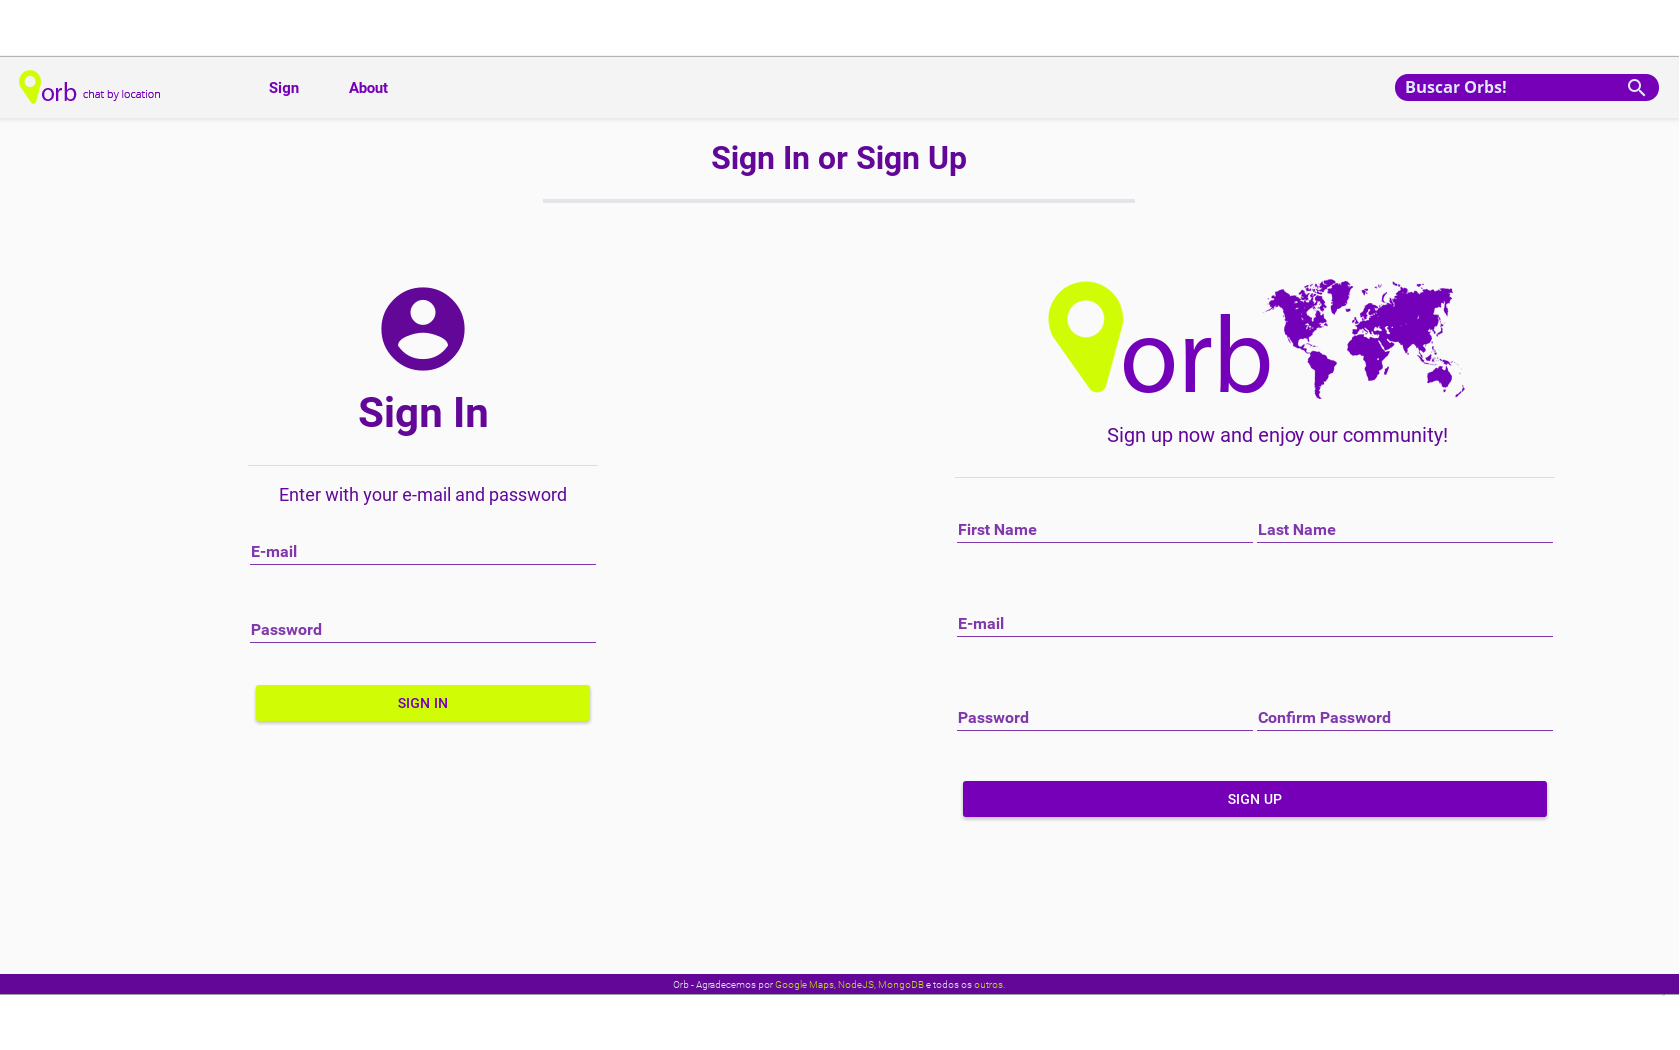
\includegraphics[scale=0.37]{imagens/pagina_signin.png}
	\caption{\small Página de acesso ao sistema.}
	\label{fig:pagina-signin}
\end{figure}

\begin{figure}[!htb]
	\centering
	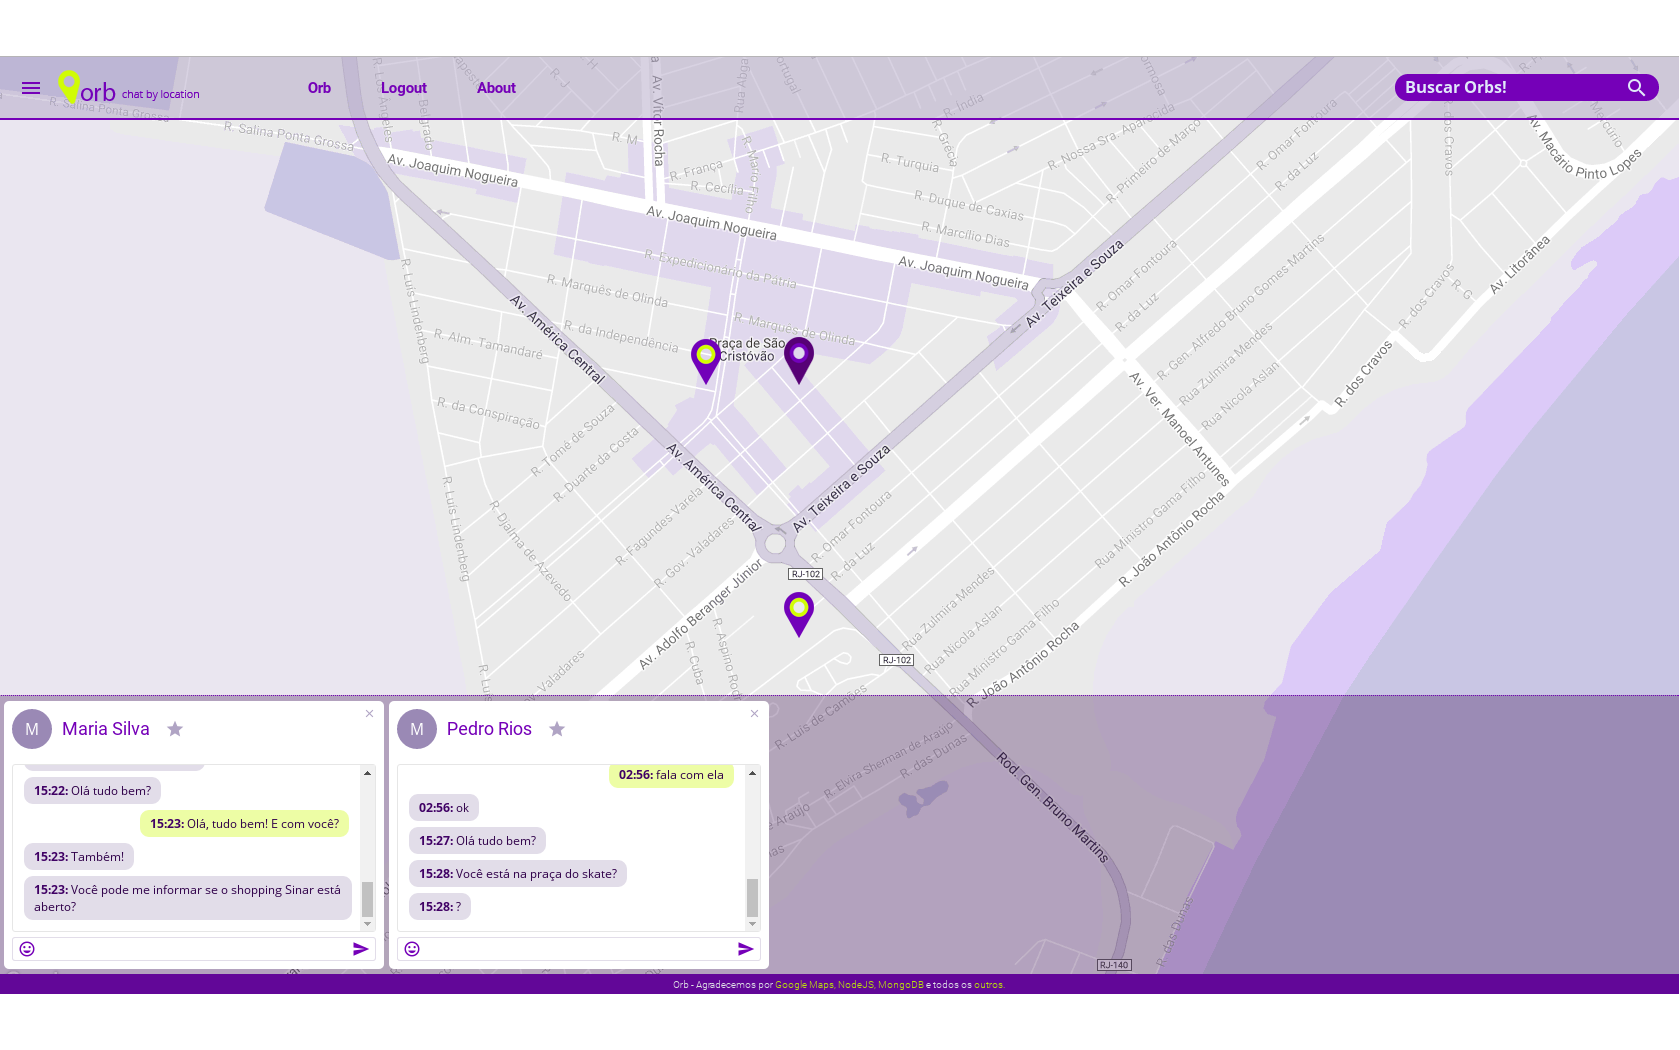
\includegraphics[scale=0.37]{imagens/pagina.png}
	\caption{\small Página principal}
	\label{fig:pagina}
\end{figure}

\begin{figure}[!htb]
	\centering
	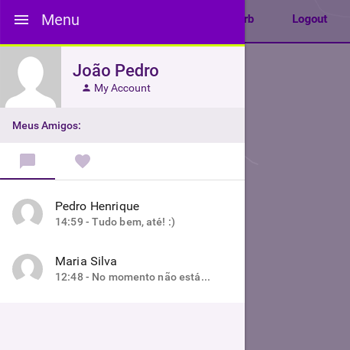
\includegraphics[scale=1]{imagens/aside_menu.png}
	\caption{\small Menu lateral}
	\label{fig:aside-menu}
\end{figure}

\begin{figure}[!htb]
	\centering
	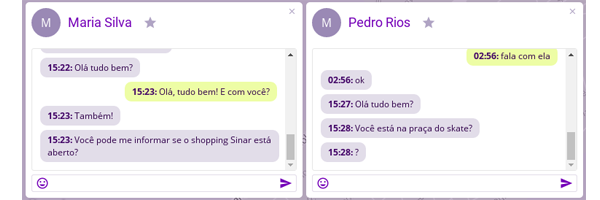
\includegraphics[scale=1]{imagens/chat_panel.png}
	\caption{\small Janelas de \textit{chat}}
	\label{fig:chat-panel}
\end{figure}
